\newpage
\section{Gas Temperatures}
\label{sec:temp}
To calculate the gas temperature we can use the formula
\begin{gather}
    \Delta \nu_D = \frac{2\nu_0}{c}\sqrt{\ln(2)\frac{2k_BT}{m}} = \frac{2\nu_0\hat{v}}{c}\sqrt{\ln(2)}~\text{with}~\hat{v}= \sqrt{\frac{2k_BT}{m}},
\end{gather}
where $\Delta\nu_D$ is the doppler width, $\nu_0$ the frequency of the peak, $\hat{v}$ the most probable velocity, $k_B$ the Boltzmann constant, $T$ the temperature and $c$ the speed of light in vacuum.
First we have to calculate the doppler width or most probable velocity. For that we are fitting a gaussian on the spectrum of the reference beam as in chapter \ref{image:gaussFit} with the form:
\begin{gather}
    y = y(\nu_0) \exp(-\left(\frac{\nu-\nu_0}{\sigma}\right)^2)
\end{gather}
With the value of $\sigma$ one can calculate $\Delta\nu_D$ or $\hat{v}$ as following:
\begin{gather}
    \Delta\nu_D = 2\sqrt{\ln(2)}\sigma \Rightarrow \sigma = \frac{\nu_0\hat{v}}{c} \Leftrightarrow \hat{v} = \frac{\sigma c}{\nu_0}
\end{gather}
After that one can obtain $T$ and the mean velocity $\overline{v}$:
\begin{gather}
    \hat{v} =  \sqrt{\frac{2k_BT}{m}} \Leftrightarrow T = \frac{m}{2 k_B} \hat{v}^2~\text{and}~\overline{v} = \sqrt{\frac{8k_BT}{\pi m}} = \sqrt{\frac{4}{\pi}}\cdot\hat{v}
\end{gather} 
We selected peak 2 for the upcoming calculation for each temperature. Because of the previous chapters \ref{sec:freeing} and \ref{sec:ratio} we know that peak 2 have to be $^{87}Rb$ and so the mass is $m\approx1.44322\cdot 10^{-25}$kg. We have transformed the laser current into frequency as in chapter \ref{sec:freeing} and with the knowledge of $\sigma$ we get following table:
\begin{center}
    \begin{tabular}{r | c c c| c c | c c}
        Temp & $\nu_0$/THz & $y(\nu_0)$/V & $\sigma$/MHz & $\hat{v}$/$\frac{m}{s}$ & $\overline{v}$/$\frac{m}{s}$& $T$/K & $T_{act}$/K\\
        \hline 
        \SI{24}{\celsius}   &384.22713 & -0.0173 & 345.26881 & 269.40 & 303.98 & 379.31 & 297,15\\ 
        \SI{38}{\celsius}   &384.22737 & -0.0313 & 361.10835 & 281.75 & 317.93 & 414.91 & 313,15\\ 
        \SI{56.2}{\celsius} &384.22724 & -0.0482 & 398.62826 & 311.03 & 350.96 & 505.62 & 329,35\\ 
    \end{tabular}
    \captionof{table}{fit parameter, velocities and temperature of the gas for each acted temperature}
\end{center}
It appears that the calculated temperatures for the gas differs from the acting temperature. But it is worth noticing that the value for $\sigma$ and so also the doppler width $\Delta\nu_D$ increases with higher temperature. In conclusion to that it gets clear that the scale of the measured values is right and that the transformation from current to frequency once again has cause problems in determine the gas temperature accurately.\\

Lastly we show in fig. \ref{image:gaussFit24}, \ref{image:gaussFit38} and \ref{image:gaussFit56} gaussian fit for each temperature.
\begin{center}
    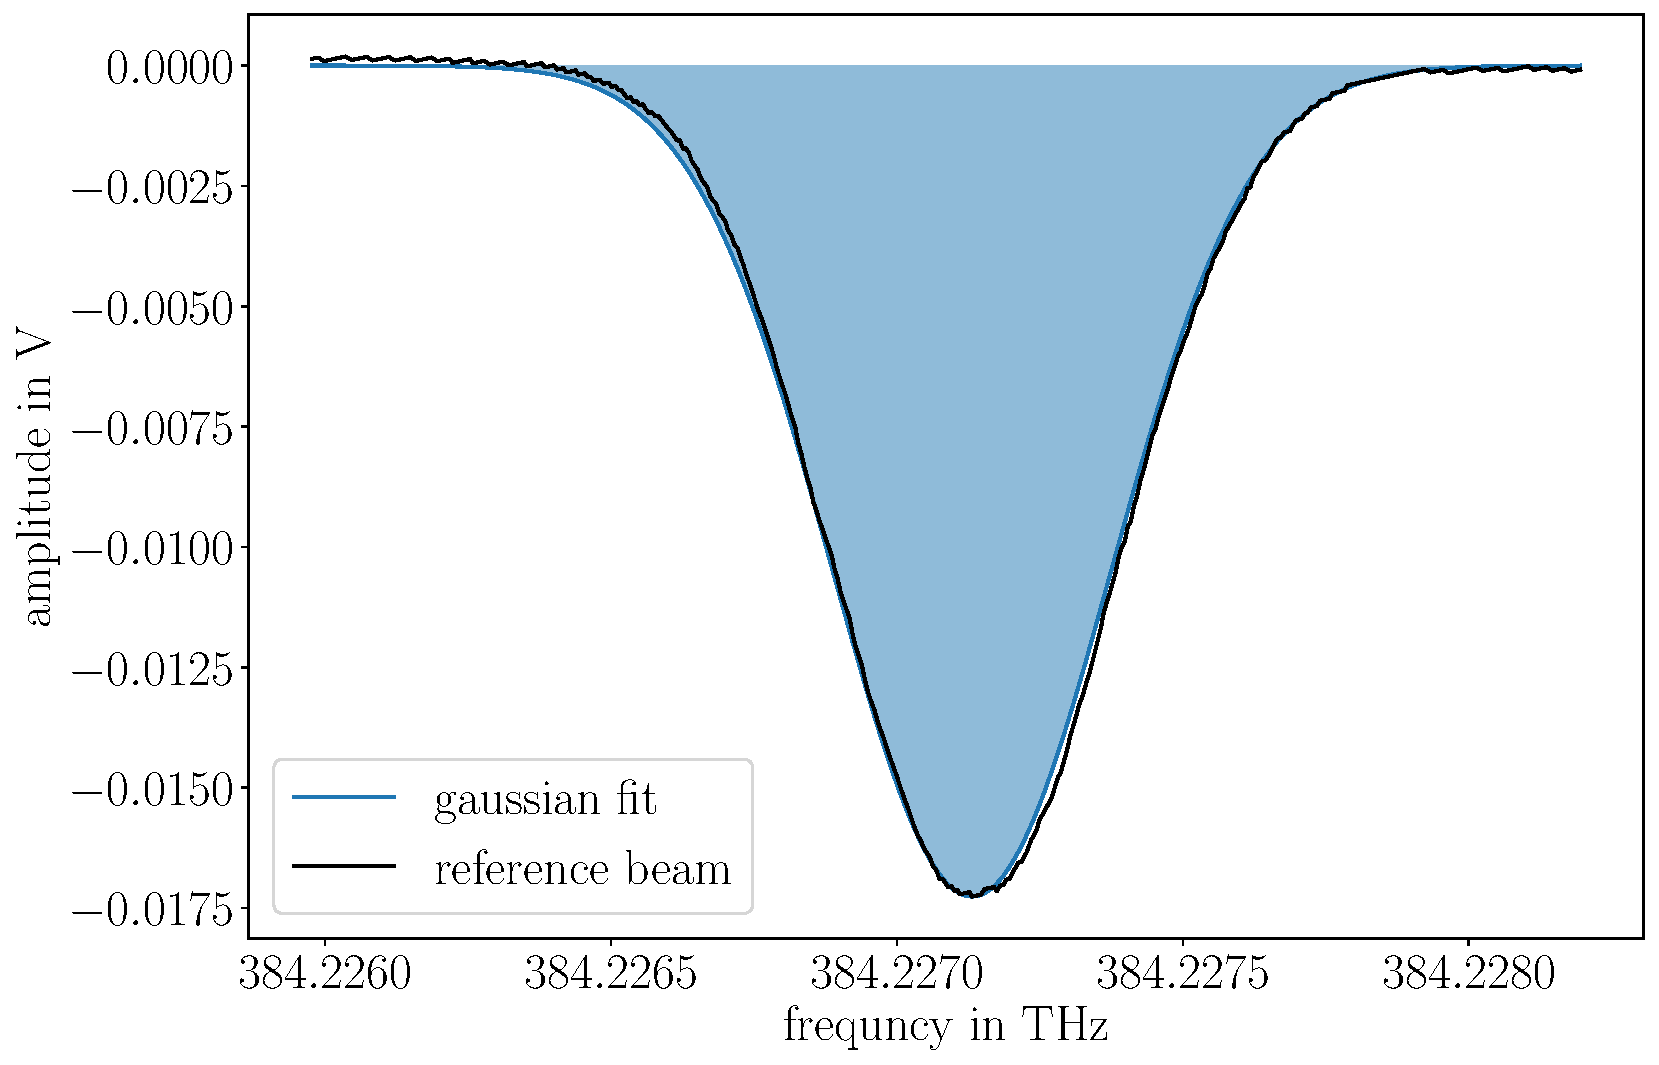
\includegraphics[scale = 0.3]{Aufg-5/gaussFitTemp24.pdf}
    \captionof{figure}{gaussian fit for temperature \SI{24}{\celsius}}
    \label{image:gaussFit24}
\end{center}
\begin{center}
    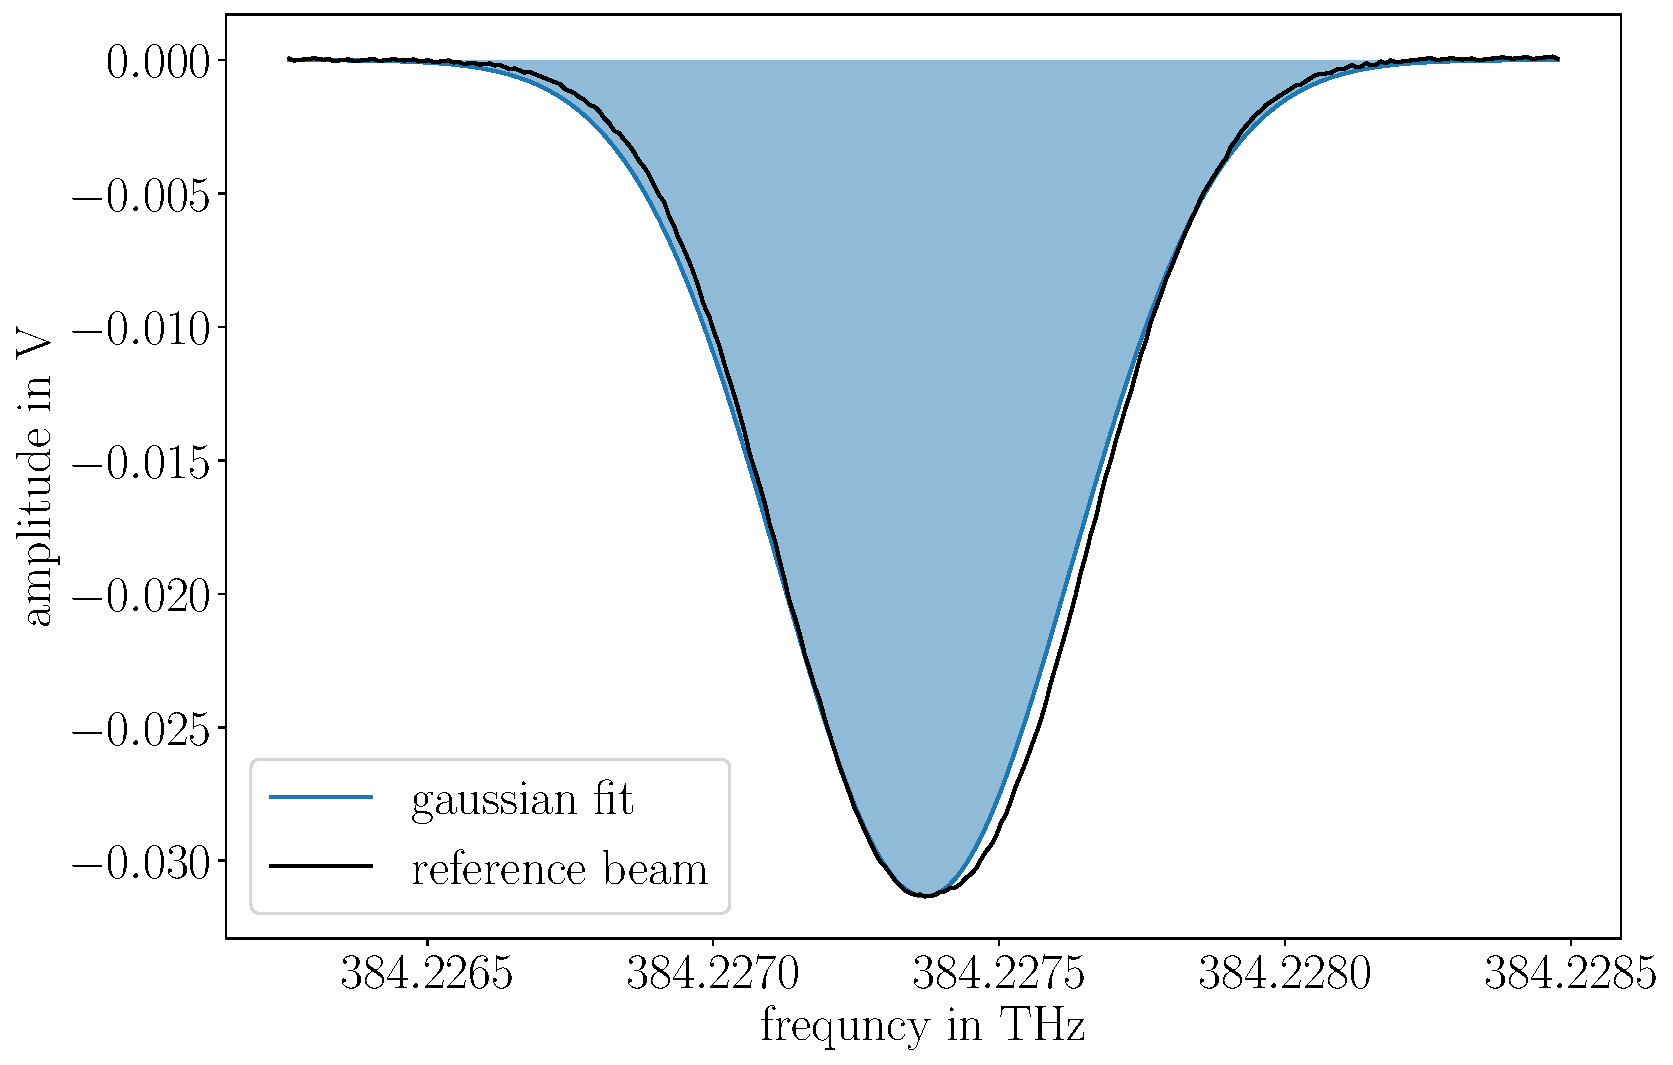
\includegraphics[scale = 0.3]{Aufg-5/gaussFitTemp38.pdf}
    \captionof{figure}{gaussian fit for temperature \SI{38}{\celsius}}
    \label{image:gaussFit38}
\end{center}
\begin{center}
    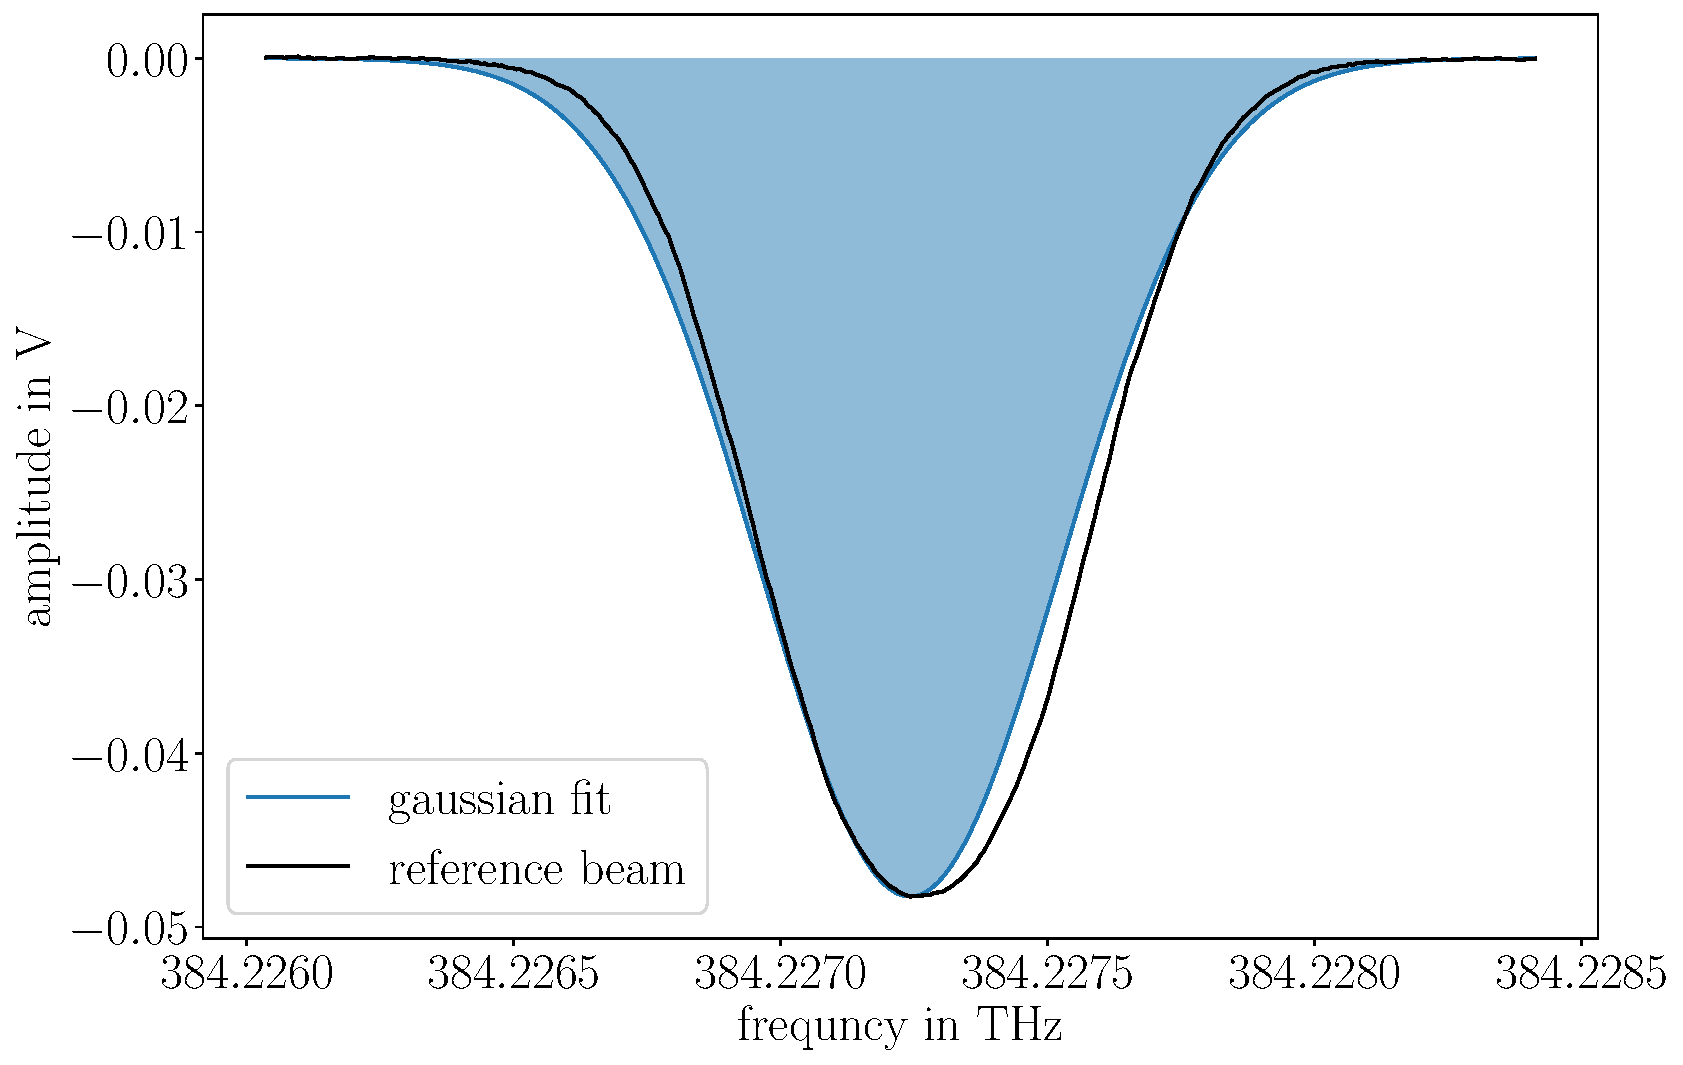
\includegraphics[scale = 0.3]{Aufg-5/gaussFitTemp56.pdf}
    \captionof{figure}{gaussian fit for temperature \SI{56.2}{\celsius}}
    \label{image:gaussFit56}
\end{center}